\documentclass[a4j,12pt,]{jarticle}
 \usepackage[dvipdfmx]{graphicx}
 \usepackage{float}
 \usepackage{siunitx} %%SI単位系用
 \usepackage{amssymb, amsmath}
 \usepackage{ascmac,here,txfonts,txfonts}
\usepackage{listings,jlisting}
\usepackage[dvipdfmx]{color}
\lstset{%
  language={Python},
  basicstyle={\small},%
  identifierstyle={\small},%
  commentstyle={\small\itshape\color[rgb]{0,0.5,0}},%
  keywordstyle={\small\bfseries\color[rgb]{0,0,1}},%
  ndkeywordstyle={\small},%
  stringstyle={\small\ttfamily\color[rgb]{1,0,1}},
  frame={tb},
  breaklines=true,
  columns=[l]{fullflexible},%
  numbers=left,%
  xrightmargin=0zw,%
  xleftmargin=3zw,%
  numberstyle={\scriptsize},%
  stepnumber=1,
  numbersep=1zw,%
  lineskip=-0.5ex%
}
\begin{document}

{\noindent\small 第9回報告書 \hfill\today}
\begin{center}
  {\Large 日射量の計算値への減衰量と相互相関が最大となるラグとの関係の調査}
\end{center}
\begin{flushright}
  祖父江匠真 \\
\end{flushright}

\section{はじめに}
今回は, 日射量の計算値に対して減衰量を掛けて実測データの概形に近づけることで, 相互相関が最大となるラグが, 減衰量を掛けなかった場合と比較して, より0 \si{\second}に近い値になるという推論の検証を行う.

\section{相互相関に使用する実測データの選定}
相互相関の計算に使用する実測値の日射量データとして, 2022年4月1日0時0分から2022年4月8日12時0分までの7.5日間を使用する.

図\ref{p1}に, 実測データを示す.

\begin{figure}[H]
  \begin{center}
    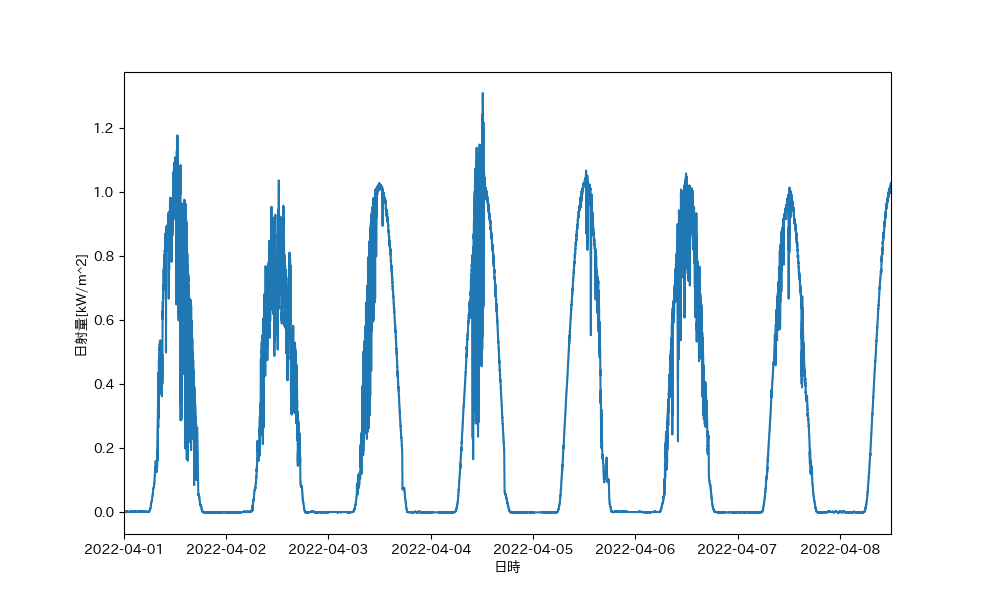
\includegraphics[width=160mm]{1.png}
    \caption{022年4月1日0時0分から2022年4月8日12時0分までの期間の実測データ}
    \label{p1}
  \end{center}
\end{figure}

図\ref{p1}の実測データに対して, 計算値の日射量データの範囲を7日間として, 1分ずつスライドさせ, そのたびに実測値データとの相互相関を計算して, 相互相関が最大となるラグを求める.
その際, 計算値全体に減衰量として0.1, 0.2, 0.3, 0.4, 0.5, 0.6, 0.7, 0.8, 0.9, 1.0のいずれかの値を掛けた上で実測値データとの相互相関を計算して, 相互相関が最大となるラグを求め, 減衰量ごとのラグを比較して, 減衰量を掛けることの有用性を検証する.

各減衰量を用いて, 相互相関を求めた結果, 全ての減衰量において, 計算値の日時を実測値より32 \si{\second}進めた際に, 相互相関の値が最大となった.
つまり, 計算値に対して, 一律で減衰量を掛けても相互相関が最大となるラグの値が変化することはないことが分かった.

図\ref{p2}に, 減衰量を1.0として計算値に掛け, 計算値を32 \si{\second}スライドさせたものと実測値を合わせてプロットしたものを示す.

\begin{figure}[H]
  \begin{center}
    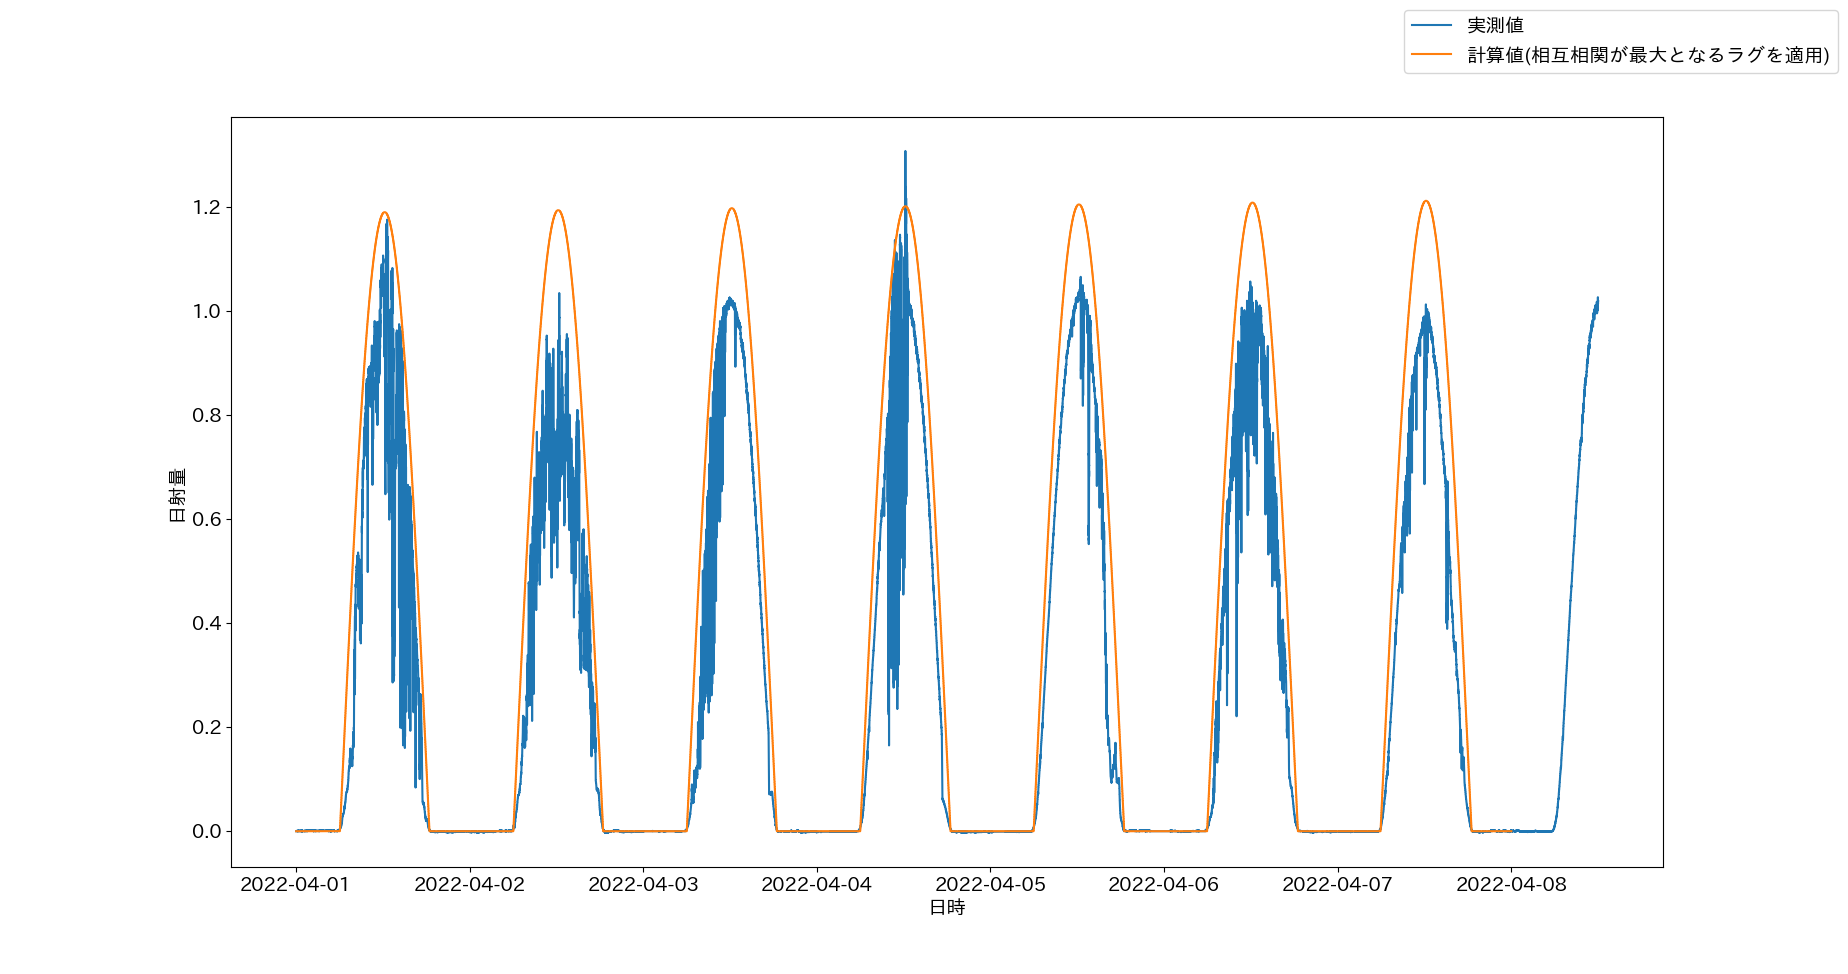
\includegraphics[width=160mm]{1.0.png}
    \caption{減衰量を1.0として計算値に掛け, 計算値を32 \si{\second}スライドさせたものと実測値を合わせてプロットしたもの}
    \label{p2}
  \end{center}
\end{figure}

図\ref{p3}に, 減衰量を0.9として計算値に掛け, 計算値を32 \si{\second}スライドさせたものと実測値を合わせてプロットしたものを示す.

\begin{figure}[H]
  \begin{center}
    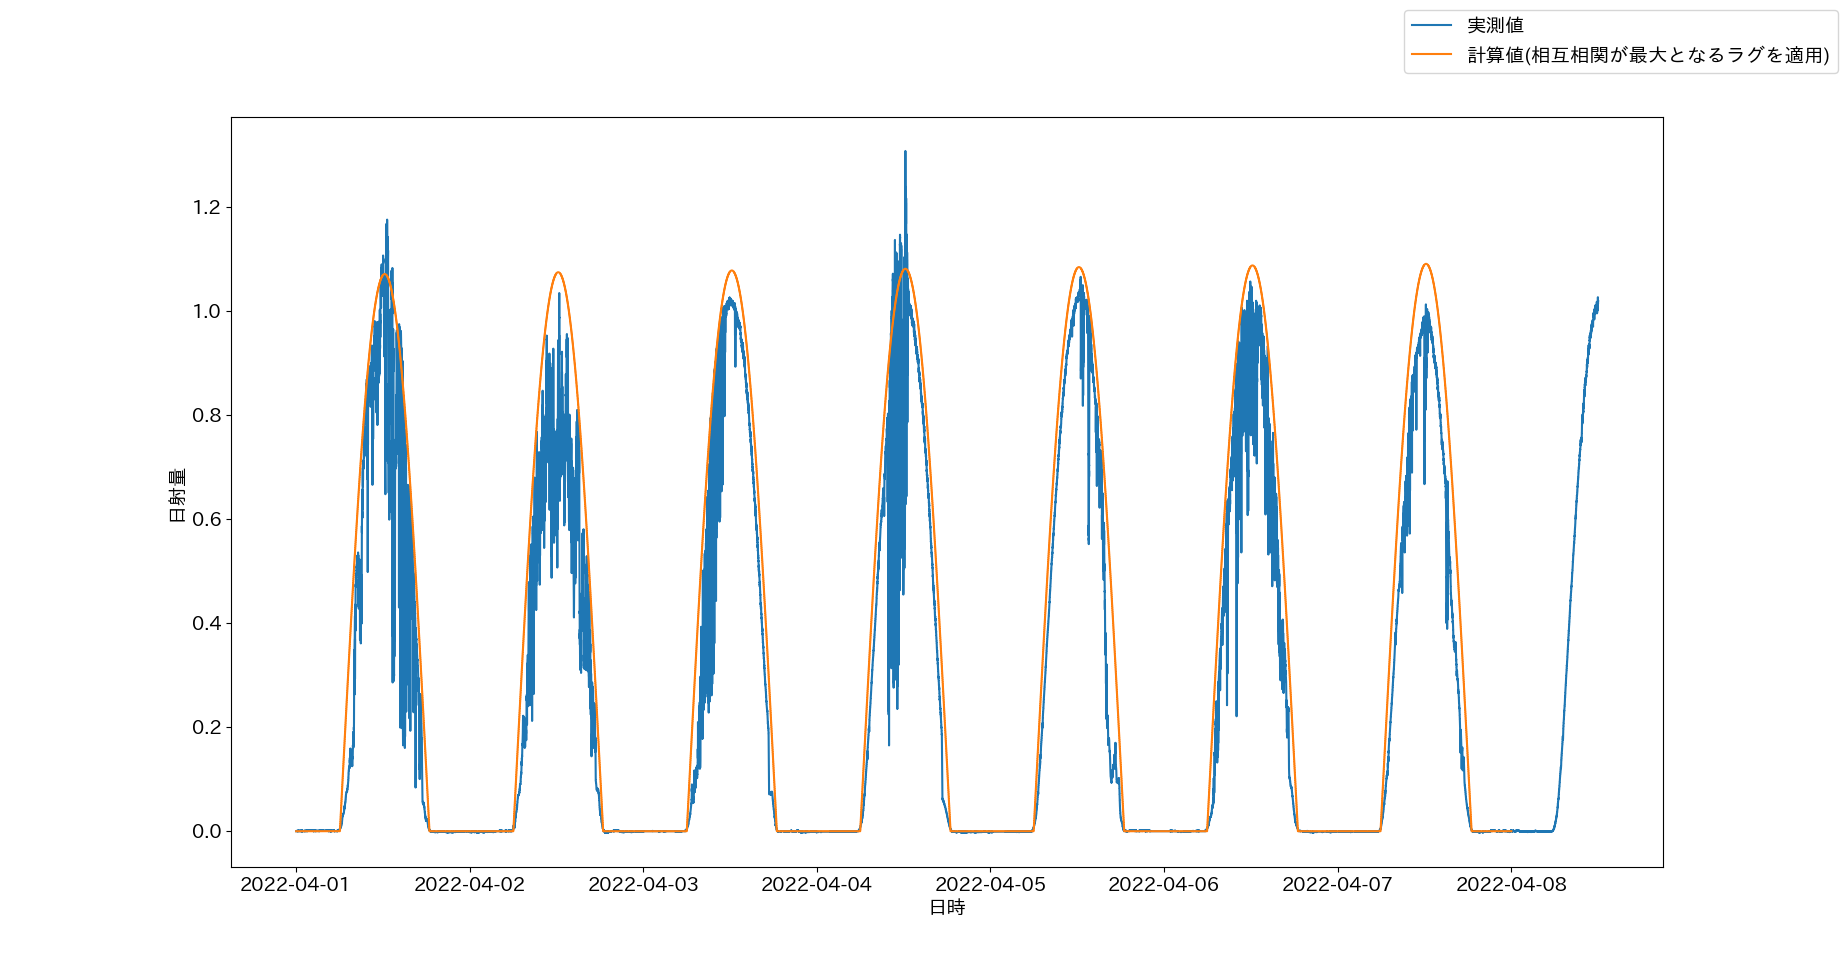
\includegraphics[width=160mm]{0.9.png}
    \caption{減衰量を0.9として計算値に掛け, 計算値を32 \si{\second}スライドさせたものと実測値を合わせてプロットしたもの}
    \label{p3}
  \end{center}
\end{figure}

図\ref{p4}に, 減衰量を0.8として計算値に掛け, 計算値を32 \si{\second}スライドさせたものと実測値を合わせてプロットしたものを示す.

\begin{figure}[H]
  \begin{center}
    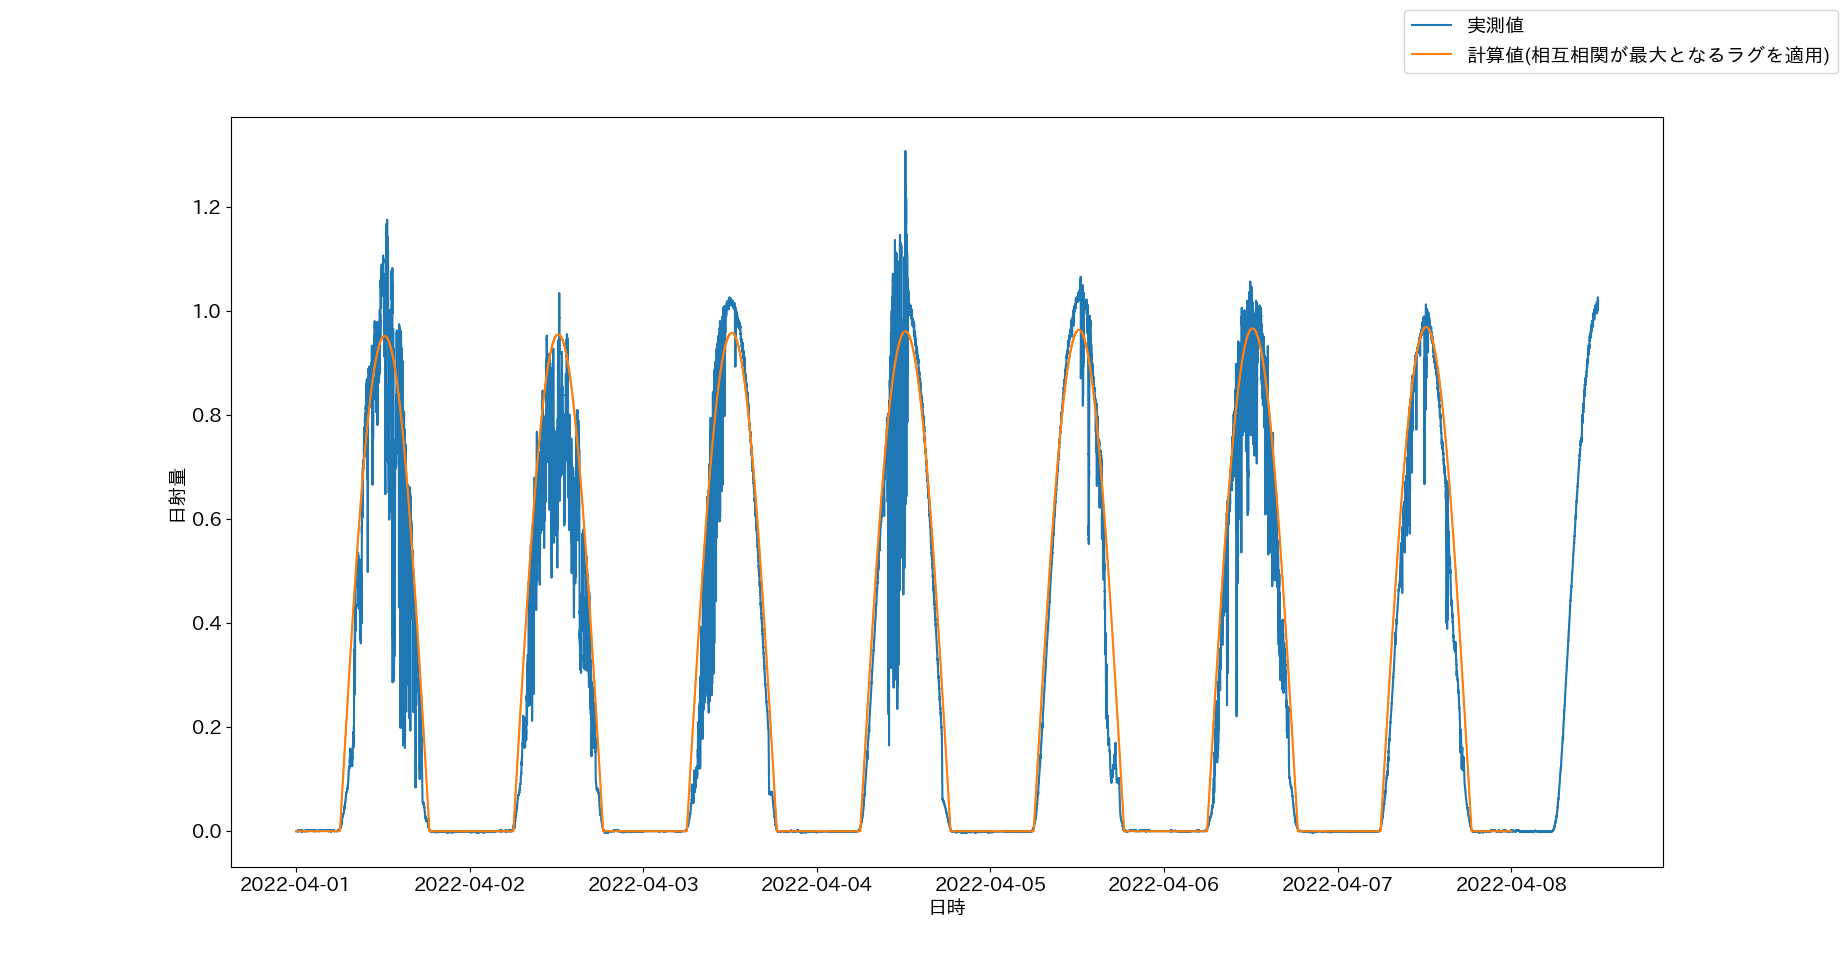
\includegraphics[width=160mm]{0.8.png}
    \caption{減衰量を0.8として計算値に掛け, 計算値を32 \si{\second}スライドさせたものと実測値を合わせてプロットしたもの}
    \label{p4}
  \end{center}
\end{figure}

図\ref{p5}に, 減衰量を0.7として計算値に掛け, 計算値を32 \si{\second}スライドさせたものと実測値を合わせてプロットしたものを示す.

\begin{figure}[H]
  \begin{center}
    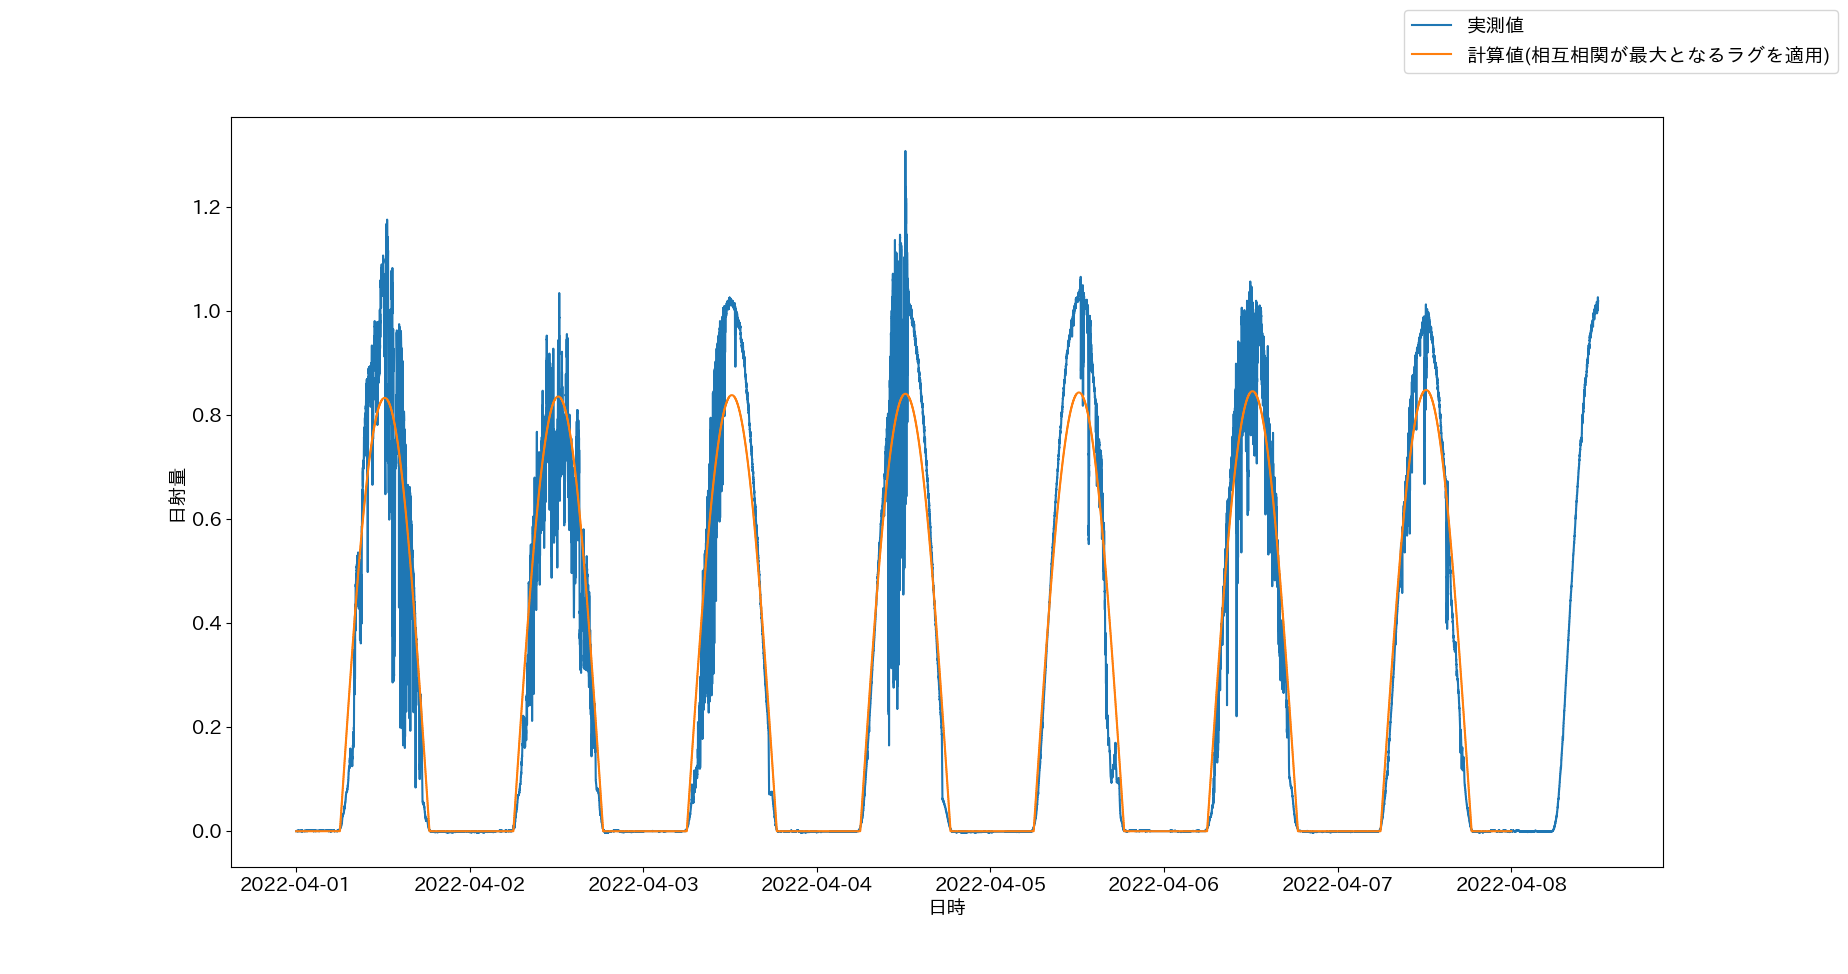
\includegraphics[width=160mm]{0.7.png}
    \caption{減衰量を0.7として計算値に掛け, 計算値を32 \si{\second}スライドさせたものと実測値を合わせてプロットしたもの}
    \label{p5}
  \end{center}
\end{figure}

図\ref{p6}に, 減衰量を0.1として計算値に掛け, 計算値を32 \si{\second}スライドさせたものと実測値を合わせてプロットしたものを示す.

\begin{figure}[H]
  \begin{center}
    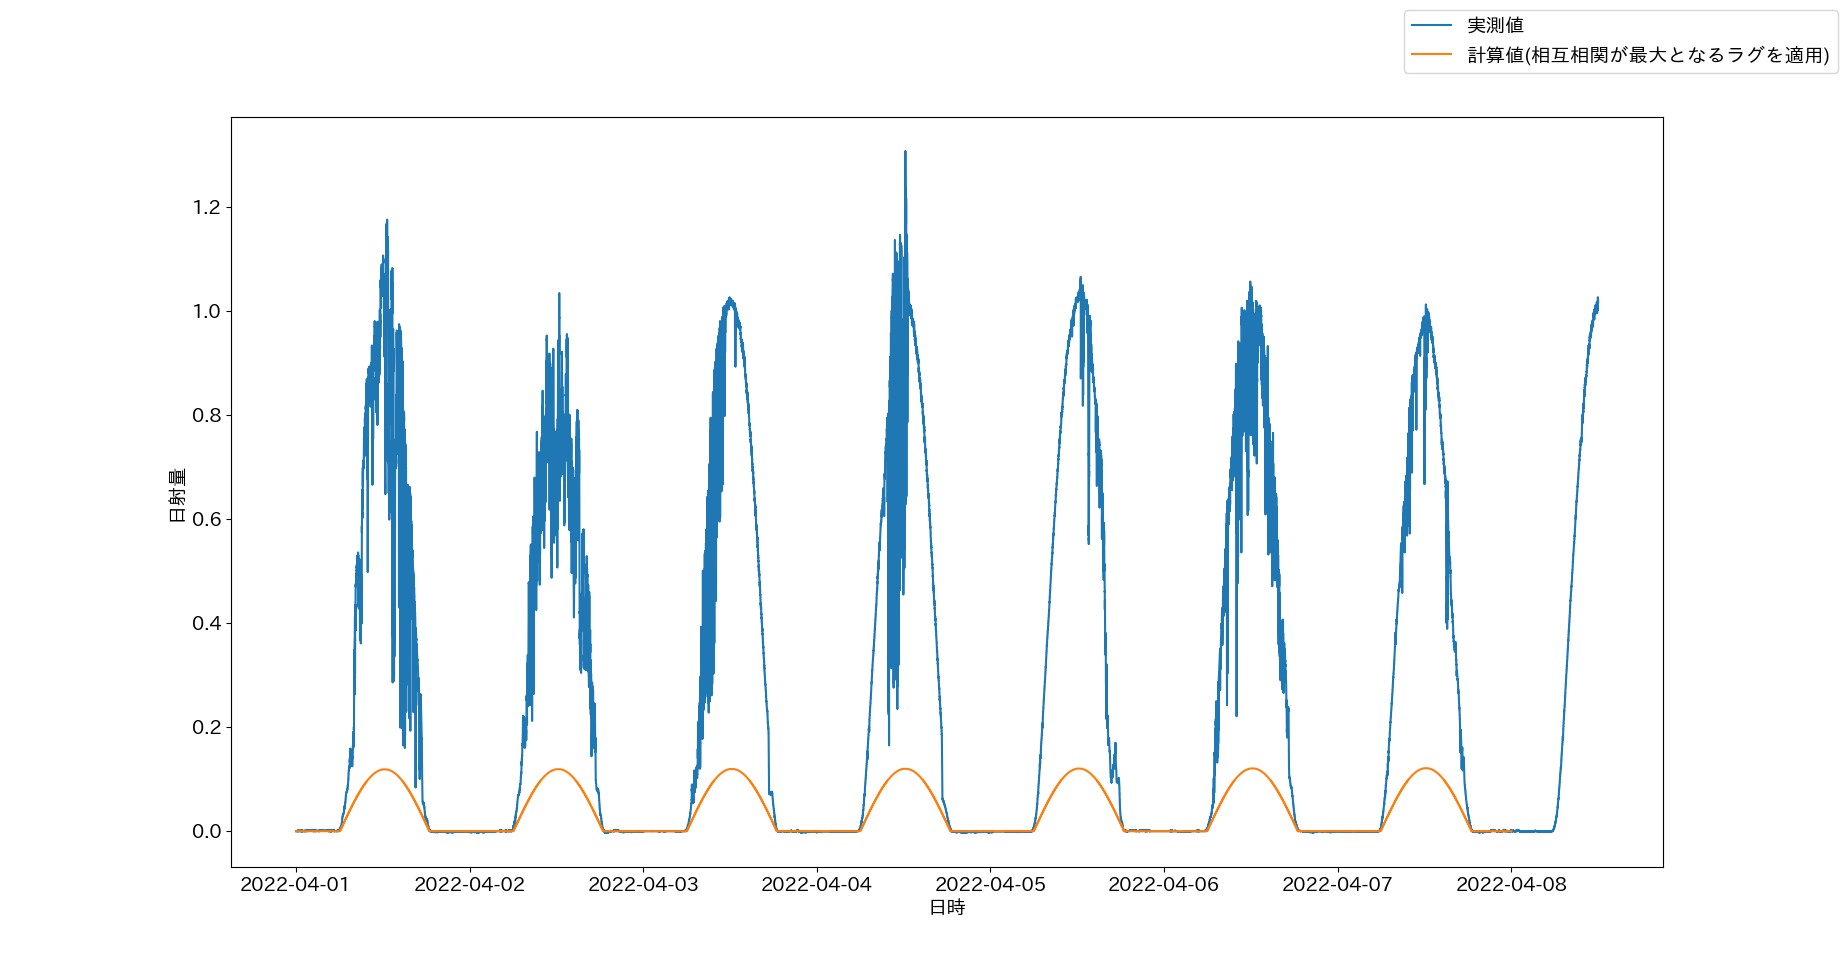
\includegraphics[width=160mm]{0.1.png}
    \caption{減衰量を0.1として計算値に掛け, 計算値を32 \si{\second}スライドさせたものと実測値を合わせてプロットしたもの}
    \label{p6}
  \end{center}
\end{figure}

\section{おわりに}
今回は, 日射量の計算値に対して減衰量を掛けて実測データの概形に近づけることで, 相互相関が最大となるラグが減衰量を掛けなかった場合と比較して, より0 \si{\second}に近い値になるという推論の検証を行った.
結果として, 計算値に対して一律で減衰量を掛けた上で相互相関を求めても, 相互相関が最大となるラグの値は減衰量間で変化せず, 計算値に対して一律の減衰量を掛けた上で相互相関を求める手法は有用ではないことが分かった.

\end{document}